% !TEX TS-program = xeLaTeX+MakeIndex+BibTeX 

\documentclass[xcolor=x11names,compress,10pt]{ctexbeamer}
\usetheme{Darmstadt} 
\useoutertheme[subsection=false,footline=authortitle]{miniframes}
\setbeamertemplate{navigation symbols}{} 
%=========================Ubuntu的字体方案==============================%
\setCJKmainfont[BoldFont={WenQuanYi Zen Hei},ItalicFont={AR PL UKai CN}]{AR PL UMing CN}
\setCJKsansfont{WenQuanYi Zen Hei}
\setCJKmonofont{WenQuanYi Micro Hei Mono}
\setCJKfamilyfont{song}{AR PL UMing CN}
\setCJKfamilyfont{kai}{AR PL UKai CN}
\setCJKfamilyfont{hei}{WenQuanYi Zen Hei}
\newcommand{\song}{\CJKfamily{song}}
\newcommand{\kai}{\CJKfamily{kai}}   
\newcommand{\hei}{\CJKfamily{hei}}




\setbeamercolor*{lower separation line head}{bg=DeepSkyBlue4} 
\setbeamercolor*{normal text}{fg=black,bg=white} 
\setbeamercolor*{alerted text}{fg=red} 
\setbeamercolor*{example text}{fg=black} 
\setbeamercolor*{structure}{fg=DeepSkyBlue4,bg=white} 

\setbeamercolor*{palette tertiary}{fg=black,bg=black!10} 
\setbeamercolor*{palette quaternary}{fg=black,bg=black!10} 

%footline
\setbeamercolor{author in head/foot}{fg=white,bg=}
\setbeamercolor{title in head/foot}{fg=white,bg=}
\setbeamercolor{date in head/foot}{fg=black,bg=}


\makeatletter
\setbeamertemplate{footline}
{%
    \setbox\beamer@tempbox=\hbox{%
        \begin{beamercolorbox}[wd=.333333\paperwidth,ht=2.25ex,dp=1ex,center]{author in head/foot}%
            \usebeamerfont{author in head/foot}\insertshortauthor
        \end{beamercolorbox}%
        \begin{beamercolorbox}[wd=.333333\paperwidth,ht=2.25ex,dp=1ex,center]{title in head/foot}%
            \usebeamerfont{title in head/foot}\insertshorttitle
        \end{beamercolorbox}%
        \begin{beamercolorbox}[wd=.333333\paperwidth,ht=2.25ex,dp=1ex,right]{date in head/foot}%
            \usebeamerfont{date in head/foot}\insertshortdate{}\hspace*{2em}
            \insertframenumber{} / \inserttotalframenumber\hspace*{2ex} 
        \end{beamercolorbox}%
    }%
    \vskip0pt%
        \begin{pgfpicture}{0pt}{0pt}{\paperwidth}{0cm}%
            \usebeamercolor{frametitle right}%
            \pgfpathrectangle{\pgfpointorigin}{\pgfpoint{\paperwidth}{3.5ex}}%
            \pgfusepath{clip}%
            \pgftext[left,base]{\pgfuseshading{beamer@frametitleshade}}%
        \end{pgfpicture}%
    \beamer@tempdim=\ht\beamer@tempbox%
    \advance\beamer@tempdim by 0.95ex%
    \vskip-\beamer@tempdim%
    \box\beamer@tempbox%
    }  
\makeatother


\colorlet{titleright}{yellow!10!white}
\colorlet{titleleft}{DeepSkyBlue4}
\colorlet{titlemid}{green!60!blue}

\makeatletter

\pgfdeclarehorizontalshading[titleleft,titleright]{beamer@frametitleshade}{\paperheight}{%
        color(0pt)=(titleleft);
        color(.5\paperwidth)=(titlemid);
        color(\paperwidth)=(titleright)
}

\AtBeginDocument{
    \pgfdeclareverticalshading{beamer@topshade}{\paperwidth}{%
        color(0pt)=(bg);
        color(4pt)=(black!50!bg)    
    }
}


\renewcommand{\(}{\begin{columns}}
\renewcommand{\)}{\end{columns}}
\newcommand{\<}[1]{\begin{column}{#1}}
\renewcommand{\>}{\end{column}}


\usepackage{graphicx}
\usepackage{mathrsfs}
\usepackage{bm}
\usepackage{comment}
\usepackage{amssymb}
\usepackage{amsfonts}
\usepackage{wrapfig}
\usepackage{subfigure}
\usepackage{media9}
\usepackage{listings}
\usepackage{hyperref}
\hypersetup{
pdfpagemode={FullScreen},
pdftitle={工欲善其事必先利其器},
pdfauthor={冷轩}
}
\newcommand{\nl}{\nonumber \\}
%\usepackage[hang]{footmisc}
%\renewcommand{\hangfootparindent}{10pt}% Indentation for 2nd etc. paragraphs in footnotes which cosists of more than one paragraph
%\renewcommand{\hangfootparskip}{3pt}% Vertical space between paragraphs in multiparagraph footnotes
%\renewcommand{\footnotemargin}{10pt}% Setting left margin; this is the smallest value I can get to have second etc. lines indented to footnote number; zero put indentation to some positive value, and negative values do not help actually
%\renewcommand{\footnotelayout}{\hspace{-2em}}% Here you can modify the spacing between the footnote number and the text of footnote; keep this value and \hangfootparindent value the same
 

\title{工欲善其事必先利其器\\——{\kai 科研工具及Python编程简介}}


\author{冷轩}
 
 
\institute
{
%  理学院  中国矿业大学(北京)
}


\CTEXoptions[today=old]
\renewcommand\figurename{Fig}
\date{\today}

%同时存在有编号和无编号脚注
\usepackage{lipsum}





\begin{document}
\maketitle

\newcommand\blfootnote[1]{% 
\begingroup 
\renewcommand\thefootnote{}\footnote{#1}% 
\addtocounter{footnote}{-1}% 
\endgroup 
}

\newenvironment{shrinkeq}[1]%缩短公式之间的距离
{ \bgroup
  \addtolength\abovedisplayshortskip{#1}
  \addtolength\abovedisplayskip{#1}
  \addtolength\belowdisplayshortskip{#1}
  \addtolength\belowdisplayskip{#1}}
{\egroup\ignorespacesafterend}

\AtBeginSection[]
{
  \begin{frame}
    \frametitle{Table of Contents}
    \tableofcontents[currentsection]%,hideallsubsections
  \end{frame}
}



\section[文献]{文献检索、跟踪与管理}
\begin{frame}{文献检索与跟踪}
\begin{figure}[htbp]
\centering

\includegraphics[width=0.8\textwidth]{pictures/1.png}
\caption{\url{https://scholar.google.com} }
%\label {fig: subfig }
\end{figure}
\end{frame}


\begin{frame}{文献检索与跟踪}
基本功能:
\begin{itemize}
\item 查看引用文章;
\item 作者文章跟踪;
\item 关键词文章跟踪;
\item 下载bib文献引用格式。
\end{itemize}
\end{frame}



\begin{frame}{文献管理工具——Zotero}
\begin{figure}[h!]
\centering
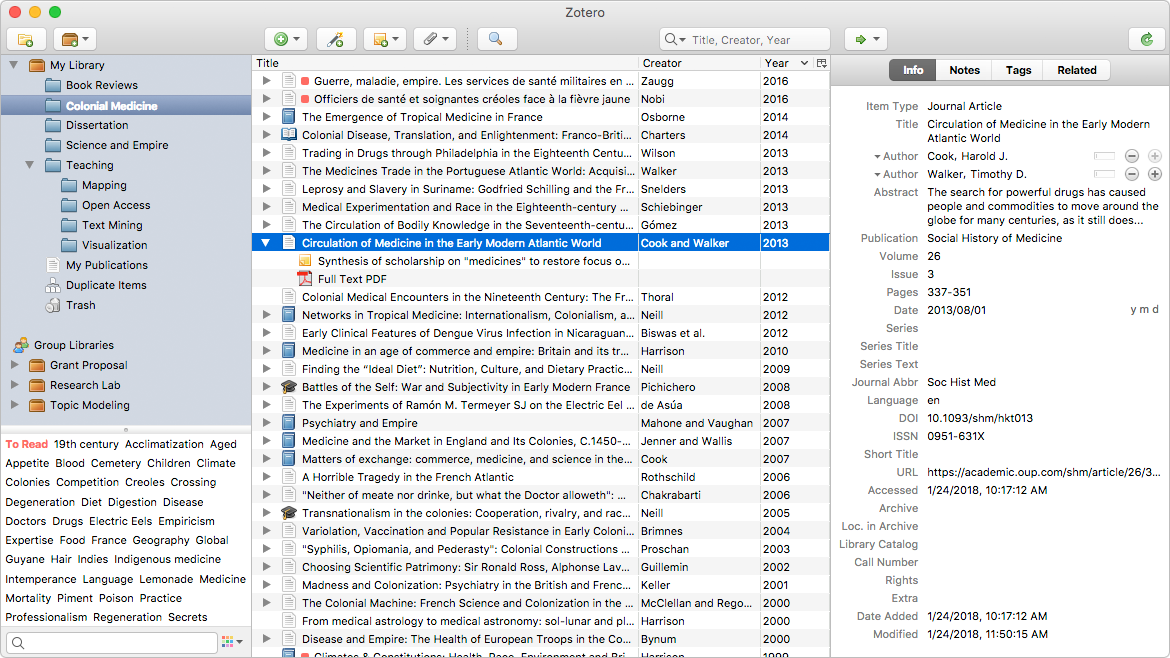
\includegraphics[width=0.8\textwidth]{pictures/zotero.png}
\caption{Zotero基本界面}
\end{figure}
\end{frame}


\begin{frame}{文献管理工具——Zotero}
基本功能:
\begin{itemize}
\item 分类与标签;
\item 文献快速下载与导入;
\item 多平台、多设备同步;
\item 文献全文检索。
\end{itemize}
\end{frame}


\section[\LaTeX]{文档写作工具——\LaTeX}
\begin{frame}{\LaTeX 历史}
\begin{itemize}
\item \TeX:一种宏语言。
\item Donald E. Knuth(高德纳)
\item TAOCP(计算机程序设计艺术; The Art of Computer Programming)
\item \LaTeX:\TeX 中的一个宏集合,是\TeX 中的一种格式 ,是建立在\TeX 基础上的宏语言,也就是说,每一个\LaTeX 命令实际上最后都会被转换解释成几个甚至上百个\TeX 命令。
\item pdf\LaTeX、 Xe\LaTeX 等:是使用\LaTeX 的排版引擎,用来编译用\LaTeX 格式写的.tex文件。
\end{itemize}
\end{frame}

\begin{frame}{\LaTeX 应用思路}
\begin{itemize}
\item 从格式上完全解放出来;
\item 特别适合进行大量的公式编辑;
\item 积累自己的成长型一手资料。
\end{itemize}
\end{frame}



\begin{frame}{\LaTeX 参考资料}
\begin{itemize}
\item \LaTeX{}模板:\url{https://github.com/ElegantLaTeX/ElegantBook}
\item 一份简短的关于\LaTeX{}安装的介绍:\url{https://github.com/OsbertWang/install-latex}
\item 一份(不太)简短的~\LaTeXe{}~介绍:\url{https://github.com/CTeX-org/lshort-zh-cn}
\item Herbert Voß*,  Mathmode: \url{http://tug.ctan.org/obsolete/info/math/voss/mathmode/Mathmode.pdf}
\end{itemize}
\end{frame}



\section[Git]{程序(文档)版本控制与协作——Git}
\begin{frame}{Git\&GitHub or Gitee}
\begin{itemize}
\item Git是程序版本控制软件,有图形界面,也有命令行界面,命令行更简单。
\item Github、Gitlab、Gitee(码云)为程序托管网络云平台。
\end{itemize}
\end{frame}



\section[Python]{Python}
\begin{frame}{学习一门编程语言的基本思路}
\begin{itemize}
\item 边用边学,在应用中学习与升级;
\item 手头备一本入门书,翻便基本语法,有个印象即可,随时查阅;
\item 一个上午完成一门编程语言的学习,可以开始上手解决自己的问题;
\item 所思即所写,充分搜索网络上自己所需的功能;
\item 程序不通过,注意查报错;
\item 中英文相结合搜索,分别上不同的搜索引擎。
\end{itemize}
\end{frame}


\begin{frame}{Python的注意事项}
\begin{itemize}
\item 一定要注意对齐,以对齐划分语言区域;
\item 注意导入自己所需的库。
\end{itemize}

优点:开源语言,全世界的人都在开发各样的库来满足人们的需求。
\end{frame}


\begin{frame}{Python的集成开发环境——Anaconda}
\begin{figure}[h!]
\centering
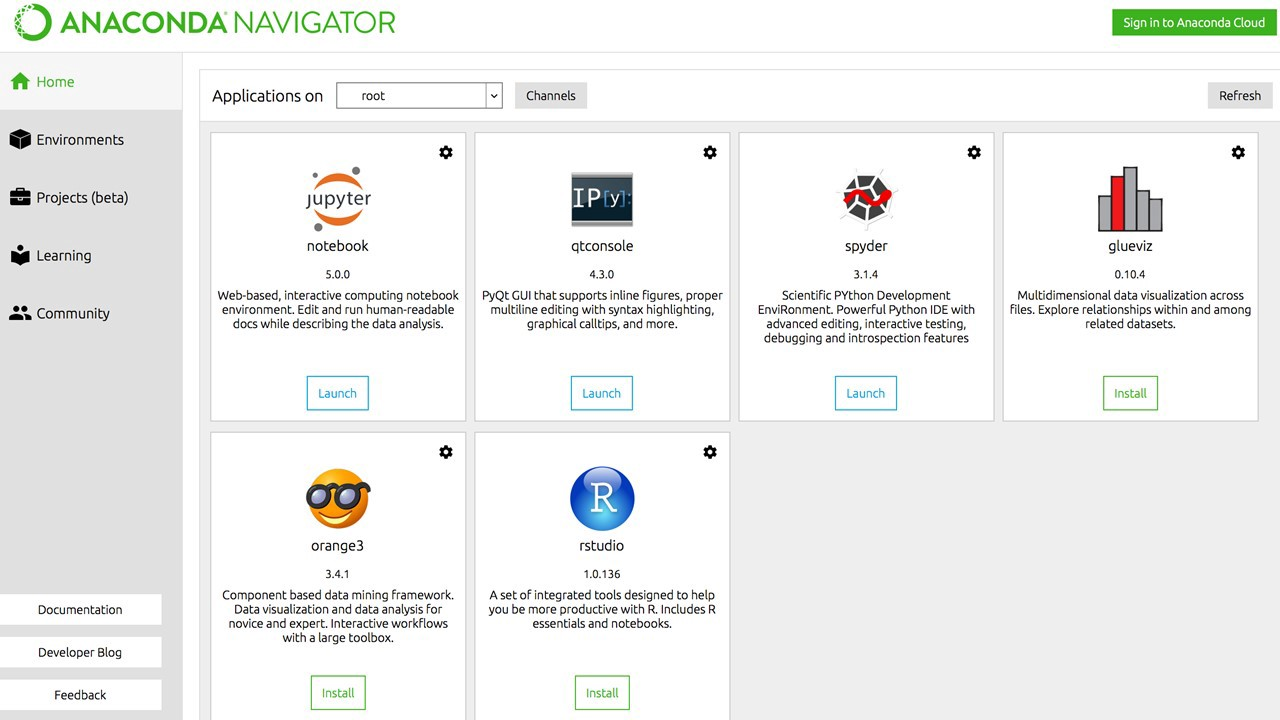
\includegraphics[width=0.8\textwidth]{pictures/anaconda.jpeg}
\caption{方便管理库}
\end{figure}
\end{frame}


\begin{frame}{Python的开发环境——Spyder}
\begin{figure}[h!]
\centering
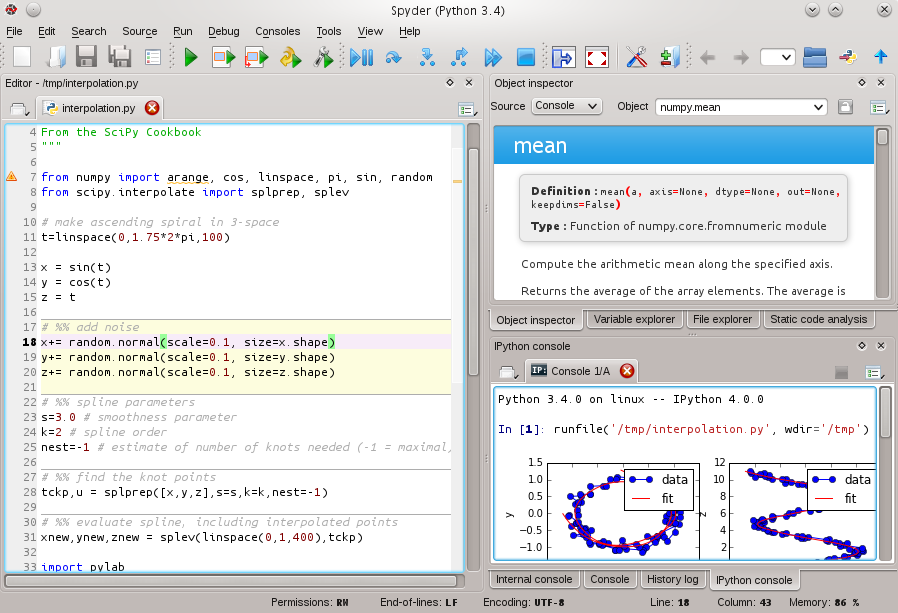
\includegraphics[width=0.8\textwidth]{pictures/Spyder.png}
\caption{和Matlab界面非常像}
\end{figure}
\end{frame}


\begin{frame}{Python的数值计算库——NumPy和SciPy}
NumPy为Python提供了快速的多维数组处理的能力,而SciPy则在NumPy基础上添加了众多的科学计算所需的各种工具包,有了这两个库,Python就有几乎和Matlab一样的处理数据和计算的能力了。
\end{frame}


\begin{frame}{Python的数据类型}
Python有五个标准的数据类型:
\begin{itemize}
\item Numbers(数字)
\item String(字符串)
\item List(列表)
\item Tuple(元组)
\item Dictionary(字典)
\end{itemize}
\end{frame}


\begin{frame}{Python程序举例}
\centering
Python程序举例
\end{frame}


\begin{frame}{参考文档}
\url{https://github.com/xuanleng/SiSR}
\end{frame}


\begin{frame}

{\huge Thank you for your attention!}

\end{frame}



\bibliographystyle{IOPthesis}
\bibliography{ref.bib}
\end{document}